勾配法は近似解を与え, 近似解の周辺の傾き等を用いて, 近似解を漸次改良し, この処理をくり返す方法である.\\
(例)\ 最急降下法, 共役勾配法, ニュートン法\\
\begin{center}
    \begin{tikzpicture}[>=stealth]
        \draw[fill=gray!20,rotate=50,xscale=1.9] (1.5,2) circle[radius=2];
        \draw[fill=gray!30,rotate=50,xscale=1.9] (1.7,2) circle[radius=1.7];
        \draw[fill=gray!40,rotate=50,xscale=1.9] (1.8,2) circle[radius=1.5];
        \draw[fill=gray!60,rotate=50,xscale=2] (1.8,2) circle[radius=1.3];
        \draw[fill=gray!70,rotate=51,xscale=2] (2,1.9) circle[radius=1];
        \draw[fill=magenta,draw=black] (-2,2) circle[radius=0.1];
        \draw(-2.1,2)--(-2.1,2) node[left]{$\mbox{\boldmath $x$}_{0}$};
        \draw[->,draw=green,very thick] (-1.9,2)--(-1.1,2);
        \node at(-1.5,1.7) {$-\nabla f(\mbox{\boldmath $x$}_{0})$};
        \node at(-1.5,1.35) {$H(\mbox{\boldmath $x$}_{0})$};
        \draw[->,draw=blue] (-1.9,2.05)--(-0.6,2.45);
        \draw[fill=magenta,draw=black] (-0.5,2.5) circle[radius=0.1];
        \draw(-0.5,2.4)--(-0.5,2.4) node[below] {$\mbox{\boldmath $x$}_{1}$};
        \draw[->,draw=green,very thick] (-0.42,2.55)--(0.32,3.55);
        \draw[->,draw=blue] (-0.42,2.55)--(1.03,3.93);
        \node at(0.8,3) {$-\nabla f(\mbox{\boldmath $x$}_{1})$};
        \node at(0.8,2.65) {$H(\mbox{\boldmath $x$}_{1})$};
        \draw[fill=magenta,draw=black] (1.1,4) circle[radius=0.1];
        \draw (1.1,4.05)--(1.1,4.05) node[above left] {$\mbox{\boldmath $x$}_{2}$};
        \draw[->,draw=green,very thick] (1.15,4.1)--(1.49,4.86);
        \draw[->,draw=blue] (1.15,4.1)--(1.84,5.17);
        \node at(2.2,4.6) {$-\nabla f(\mbox{\boldmath $x$}_{2})$};
        \node at(2.2,4.25) {$H(\mbox{\boldmath $x$}_{2})$};
        \draw[fill=red] (1.9,5.3) circle[radius=0.15];
        \node at(-2.3,3) {適当な初期値};
    \end{tikzpicture}
\end{center}
このように近似解を繰り返し修正することで最適値へ近づいていく. 勾配(, ヘシアン), つまり$E$の$\mbox{\boldmath $x$}_{0}$における1次(,2次)の微分)施すことで修正を行う. \\
問題としては近似解の精度を上げるために\textcolor{red}{どちらの方向にどれだけ}動かすか?ということである.
\subsubsection{最急降下法}
最急降下法は最も単純なもので勾配の方向に適当量移動させるという方法である. 式にすると以下のように表すことができる.
\begin{align*}
    x_{i+1}=x_{i}-\alpha \nabla f(\mbox{\boldmath $x$}_{i}) \tag{3.4}
\end{align*}
イメージ図としては以下のようになる.
\begin{center}
    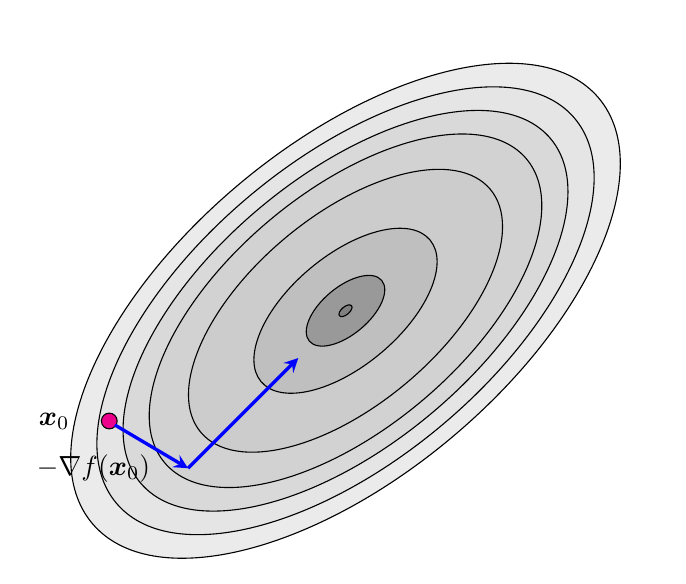
\begin{tikzpicture}[>=stealth]
        \draw[rotate=40,fill=gray!16,xscale=2] circle[radius=2.1];
        \draw[rotate=40,fill=gray!20,xscale=2] circle[radius=1.9];
        \draw[rotate=40,fill=gray!30,xscale=2] circle[radius=1.7];
        \draw[rotate=40,fill=gray!35,xscale=2] circle[radius=1.5];
        \draw[rotate=40,fill=gray!40,xscale=2] circle[radius=1.2];
        \draw[rotate=40,fill=gray!50,xscale=2] circle[radius=0.7];
        \draw[rotate=40,fill=gray!80,xscale=2] circle[radius=0.3];
        \draw[rotate=40,fill=gray,xscale=2] circle[radius=0.05];
        \draw[fill=magenta] (-3,-1.4) circle[radius=0.1];
        \draw[->,very thick,draw=blue] (-2.93,-1.45)--(-2,-2);
        \draw[->,very thick,draw=blue] (-2,-2)--(-0.6,-0.6);
        \node at(-3.2,-2) {$-\nabla f(\mbox{\boldmath $x$}_{0})$};
        \node at(-3.7,-1.4) {$\mbox{\boldmath $x$}_{0}$};
    \end{tikzpicture}
\end{center}
誤差が最小となるところに持っていく. ということは誤差関数において値が最小となるように持ってくることである. つまり誤差関数の現時点にいる場所から傾きを得る. それが負であれば$+$にずらし, 正なら$-$にずらすことで最小値に近づけることが可能となる. 誤差関数が二次関数においての例は以下である.
\begin{center}
    \begin{tikzpicture}[>=stealth]
    \draw[very thick,domain=-3:3] plot(\x,{\x*\x/2});
    \draw[->] (-3,0)--(3,0) node[right] {$x$};
    \draw[->] (0,-0.3)--(0,5) node[above] {$y$};
    \node at(-0.2,-0.2) {O};
    \draw[thick,domain=1.5:2.5,draw=red] plot(\x,{2*\x-2});
    \draw[fill=magenta] (2,2) circle[radius=0.08];
    \draw[fill=magenta] (-2,2) circle[radius=0.08];
    \node at(4.3,2) {傾きが$+$なので$-$方向へ};
    \draw[thick,domain=-2.5:-1.5,draw=red] plot(\x,{-2*\x-2});
    \node at(-4.3,2) {傾きが$-$なので$+$方向へ};
    \end{tikzpicture}
\end{center}
最急降下法のアルゴリズムは以下のように表すことができる.\\[0.1cm]
$i_{0},\ x_{0}$を決める.\\
収束するまで繰り返し\{\\
\hspace{1cm} $x_{i+1}=x_{i}-\alpha \nabla f(\mbox{\boldmath $x$}_{i})$\\
\hspace{1cm} $i=i+1$\\
\}\\[0.1cm]
$\alpha$の決め方は様々であり, $-\nabla f(\mbox{\boldmath $x$})$の最適値を解析的に求めるかラインサーチによって求めて移動する. このときの移動量は同じであるが過去の勾配の大きさの履歴に応じて移動量を決定する.
\begin{center}
    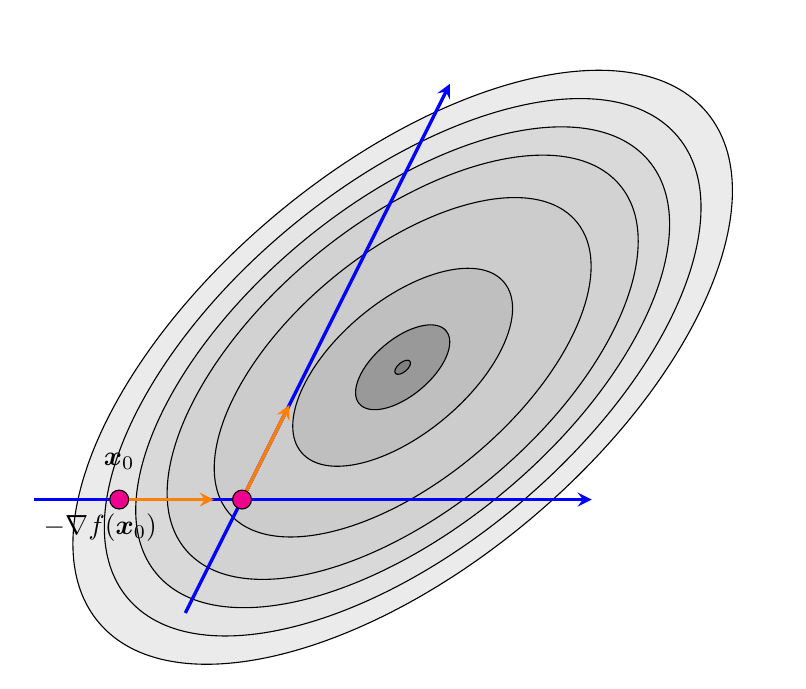
\begin{tikzpicture}[scale=1.2,>=stealth]
        \draw[rotate=40,fill=gray!16,xscale=2] circle[radius=2.1];
        \draw[rotate=40,fill=gray!20,xscale=2] circle[radius=1.9];
        \draw[rotate=40,fill=gray!30,xscale=2] circle[radius=1.7];
        \draw[rotate=40,fill=gray!35,xscale=2] circle[radius=1.5];
        \draw[rotate=40,fill=gray!40,xscale=2] circle[radius=1.2];
        \draw[rotate=40,fill=gray!50,xscale=2] circle[radius=0.7];
        \draw[rotate=40,fill=gray!80,xscale=2] circle[radius=0.3];
        \draw[rotate=40,fill=gray,xscale=2] circle[radius=0.05];
        \draw[->,very thick,draw=blue] (-3.9,-1.4)--(2,-1.4);
        \draw[->,very thick,draw=blue] (-2.3,-2.6)--(0.5,3);

        \draw[->,very thick,draw=orange](-1.7,-1.4)--(-1.2,-0.4); 
        \draw[fill=magenta] (-3,-1.4) circle[radius=0.1];
        \draw[fill=magenta] (-1.7,-1.4) circle[radius=0.1];
        \node at(-3.2,-1.7) {$-\nabla f(\mbox{\boldmath $x$}_{0})$};
        \node at(-3,-1) {$\mbox{\boldmath $x$}_{0}$};
        \draw[->,very thick,draw=orange](-2.9,-1.4)--(-2,-1.4);
    \end{tikzpicture}
\end{center}
以下の関数の最小値を最急降下法で求めてみる.
\begin{eqnarray*}
    f(\mbox{\boldmath $x$}) = \frac{1}{2}\mbox{\boldmath $x$}^{T}\begin{pmatrix}6&1\\1&2\end{pmatrix}\mbox{\boldmath $x$}-\begin{pmatrix}2\\1\end{pmatrix}^{T}\mbox{\boldmath $x$}
\end{eqnarray*}
これの初期値として$\mbox{\boldmath $x$}=\begin{pmatrix}0\\0\end{pmatrix}$としてpythonで実装した場合は以下のようになる.
\lstinputlisting{grad.py}

実行結果として, 最小値は$\begin{pmatrix}0.27281847\\0.36325003\end{pmatrix}$が得られる.\\
$\alpha$の値を移動量を最初大きくし, 最適解に近づくにつれてだんだん小さくした場合のpythonの実装は以下のようになる.
\lstinputlisting{grad2.py}
実行結果として, 最小値は$\begin{pmatrix}0.27279382\\0.36320777\end{pmatrix}$が得られる.\\[1cm]
関数$\displaystyle f(x)=\frac{1}{2}\mbox{\boldmath $x$}^{T}A\mbox{\boldmath $x$}-\mbox{\boldmath $b$}^{T}\mbox{\boldmath $x$}$の最小値を与える$\alpha$について解析的に求める方法はまず変数$\mbox{\boldmath $x$}$について
\begin{eqnarray*}
    \mbox{\boldmath $x$} = \mbox{\boldmath $x$}_{0}+\alpha \mbox{\boldmath $d$}
\end{eqnarray*}
とおき, これを代入することで計算していく.
まず
\begin{eqnarray*}
    f(x) &=& f(\mbox{\boldmath $x$}_{0}+\alpha\mbox{\boldmath $d$})\\
    f(\alpha) &=& \frac{1}{2}(\mbox{\boldmath $x$}_{0}+\alpha \mbox{\boldmath $d$})^{T}A(\mbox{\boldmath $x$}_{0}+\alpha \mbox{\boldmath $d$})-\mbox{\boldmath $b$}^{T}(\mbox{\boldmath $x$}_{0}+\alpha \mbox{\boldmath $d$})
\end{eqnarray*}
最小値を与える$\alpha$であるので極値を求めればよく,
\begin{eqnarray*}
    \frac{d}{d\alpha}f(\alpha) = 0
\end{eqnarray*}
が成立すればよい.
したがってこれを計算すると
\begin{eqnarray*}
    &&\frac{d}{d\alpha}f(\alpha) = 0\\
    \Longleftrightarrow \ && (\mbox{\boldmath $x$}_{0}+\alpha \mbox{\boldmath $d$})^{T}A\mbox{\boldmath $d$}-\mbox{\boldmath $b$}^{T}\mbox{\boldmath $d$} = 0\\
    \Longleftrightarrow\ && \alpha \mbox{\boldmath $d$}^{T}A\mbox{\boldmath $d$}+\mbox{\boldmath $x$}_{0}^{T}A\mbox{\boldmath $d$}-\mbox{\boldmath $b$}^{T}\mbox{\boldmath $d$} = 0\\
    \Longleftrightarrow \ && \alpha \mbox{\boldmath $d$}^{T}A\mbox{\boldmath $d$}+\nabla f(\mbox{\boldmath $x$}_{0})^{T}\mbox{\boldmath $d$}=0\\
    \Longleftrightarrow\ && \alpha = -\frac{\nabla f(\mbox{\boldmath $x$}_{0})^{T}\mbox{\boldmath $d$}}{\mbox{\boldmath $d$}^{T}A\mbox{\boldmath $d$}}
\end{eqnarray*}